\documentclass[10pt]{article}
\usepackage[a4paper,margin=2cm]{geometry}
\usepackage{amsmath}
\usepackage{booktabs}
\usepackage{graphicx}
\usepackage{caption}
\usepackage{enumitem}
\usepackage{float}
\usepackage[hidelinks]{hyperref}
\setlist{nosep,leftmargin=1.2em}
\captionsetup{font=small,labelfont=bf}
\setlength{\parskip}{3pt}
\setlength{\parindent}{0pt}
\begin{document}
\begin{center}
{\Large\bfseries AI651 -- Deep Learning for Space, Time and Graphs}\\[2pt]
{\large Assignment 1}\\[6pt]
Muhammad Sohaib Shahzad \quad Roll number: \textbf{27100078}\\[2pt]
GitHub repository: \url{https://github.com/chmuhammadsohaib/DL4STG-PA1}
\end{center}

\section{Task 1 -- Forecasting across heterogeneous sensors}
\begin{itemize}
\item I ran the notebook with \texttt{PA1\_PRESET=full} on a Kaggle GPU, and all the numbers below come from that run. All notebook checks passed with my three cells.
\item Unless I say otherwise, numbers are on the validation split. RMSE is in m/s$^2$ and MSE in (m/s$^2$)$^2$.
\item I included the figures below, and they are also submitted seperately as PDFs with the same output numbers and file names.
\end{itemize}

\begin{table}[H]\centering\small
\begin{tabular}{lrrrrrrrr}
\toprule
& \multicolumn{4}{c}{Established stations 1--3} & \multicolumn{4}{c}{Held-out station 4} \\
\cmidrule(lr){2-5}\cmidrule(lr){6-9}
Model & all & A & B & C & all & A & B & C \\
\midrule
Shared ridge & 0.767 & 0.805 & 0.854 & 0.621 & 0.876 & 0.909 & 0.982 & 0.713 \\
Sensor-specific ridge & 0.768 & 0.804 & 0.852 & 0.630 & -- & -- & -- & -- \\
Period-routed ridge & 0.166 & 0.181 & 0.164 & 0.152 & 0.173 & 0.184 & 0.182 & 0.150 \\
Raw Attention & 0.432 & 0.419 & 0.461 & 0.416 & 0.649 & 0.650 & 0.618 & 0.678 \\
\bottomrule
\end{tabular}
\caption{Output 1.1: validation RMSE by population and product.}\label{tab:o11}
\end{table}

\subsection*{Response 1A}
\textbf{Expectations (written down before running Output 1.1)}
\begin{itemize}
\item Established stations: period-routed ridge $<$ Raw Attention $<$ shared ridge $<$ sensor-specific ridge.
\item Station 4: period-routed ridge $<$ Raw Attention $<$ shared ridge (there is no sensor-specific model for station 4).
\item Products: the biggest errors on Product A, for the models that can't pin down the exact pace.
\end{itemize}
\textbf{Measurements (Table~\ref{tab:o11})}
\begin{itemize}
\item The order held on both populations. Established: 0.166 $<$ 0.432 $<$ 0.767 $\approx$ 0.768. Station 4: 0.173 $<$ 0.649 $<$ 0.876.
\item Compared to shared ridge, period routing cuts the RMSE by 78\% on the established stations and by 80\% on station 4. Raw Attention only cuts it by 44\% and 26\%.
\item On the established stations, sensor-specific ridge is no better than shared ridge (0.768 vs.\ 0.767).
\item Moving to station 4 makes routed ridge 4\% worse, shared ridge 14\% worse and Raw Attention 50\% worse.
\item Products, established stations: routed ridge is worst on A (0.181, then B 0.164 and C 0.152), but shared ridge, sensor-specific ridge and Raw Attention are all worst on B (0.854, 0.852 and 0.461). On station 4, shared ridge is again worst on B (0.982), but Raw Attention is worst on C (0.678).
\end{itemize}
\textbf{Revised expectations}
\begin{itemize}
\item The order of the models stays the same.
\item But routed ridge beats Raw Attention by a lot more than I thought: 2.6$\times$ on the established stations and 3.8$\times$ on station 4.
\item On the established stations, the non-routed models are worst on Product B, not A. There are only five validation runs per product, so I think this depends on which paces were drawn as much as on each product's pace range.
\end{itemize}
\textbf{Why, based on what each model assumes}
\begin{itemize}
\item \emph{Shared ridge} uses one linear map for every window. It has to average how windows with different paces carry on, and averaging cycles that are out of step makes them flatter (see 1B).
\item \emph{Sensor-specific ridge} picks its map by station, but the pace changes inside every station. So each map has the same problem, with a third of the data.
\item \emph{Period-routed ridge} picks its map by the pace, which is the thing that actually changes. Inside a 1.5-sample band, one linear rule is almost right. Since it's linear, it also scales exactly to station 4's bigger vibration, and subtracting the last value of the context (anchoring) removes station 4's offset.
\item \emph{Raw Attention} builds its mixing from the window itself, which is why it beats shared ridge. But it has to learn how to read the pace from the training windows while the drift ramp makes up most of its input. Its non-linear map was also fitted only on stations 1--3, which may explain part of its 50\% jump on station 4.
\end{itemize}

\subsection*{Response 1B}
\begin{figure}[H]\centering
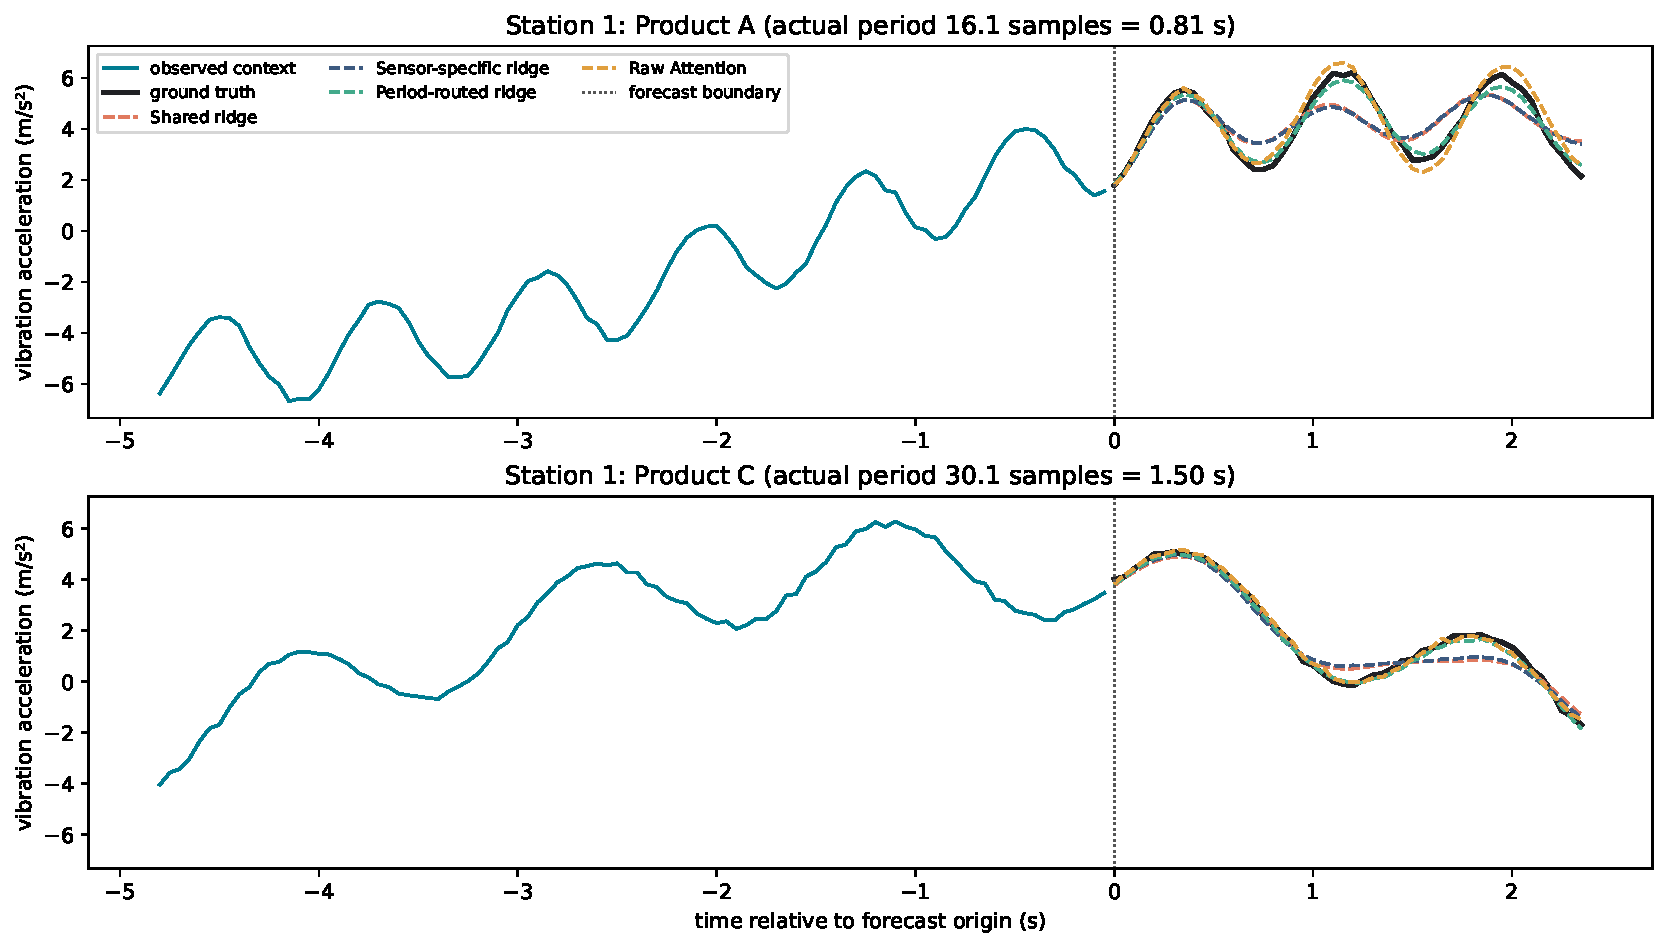
\includegraphics[width=0.92\linewidth]{figures/1.2-1.pdf}
\caption{Output 1.2: two validation windows from station 1, Product A ($P=16.1$) and Product C ($P=30.1$).}
\end{figure}
\textbf{Why one $\widehat W$ has to compromise} (Output 1.2, \texttt{1.2-1.pdf}: two validation windows from station 1, Product A with $P=16.1$ and Product C with $P=30.1$)
\begin{itemize}
\item In both windows, shared ridge gives \emph{damped} forecasts.
\item Product A: the first cycle is in phase, but later peaks only reach about 5\,m/s$^2$ instead of 6.2, and the troughs stay near 3.5 instead of 2.4.
\item Product C: the trough at 1.0--1.5\,s gets filled in (about 0.5--0.8 instead of 0).
\item The reason is that $\widehat W$ in Eq.~(8) is one least-squares fit over windows of every pace. Two contexts can look almost the same over 96 samples, but if their paces differ, what comes next drifts apart by $2\pi h(1/P_1-1/P_2)$ over the horizon.
\item The single map with the lowest MSE then returns something like their average. Averaging cycles that are out of step partly cancels them, so the forecast is damped after the first cycle and its shape gets smoothed.
\end{itemize}
\begin{figure}[H]\centering
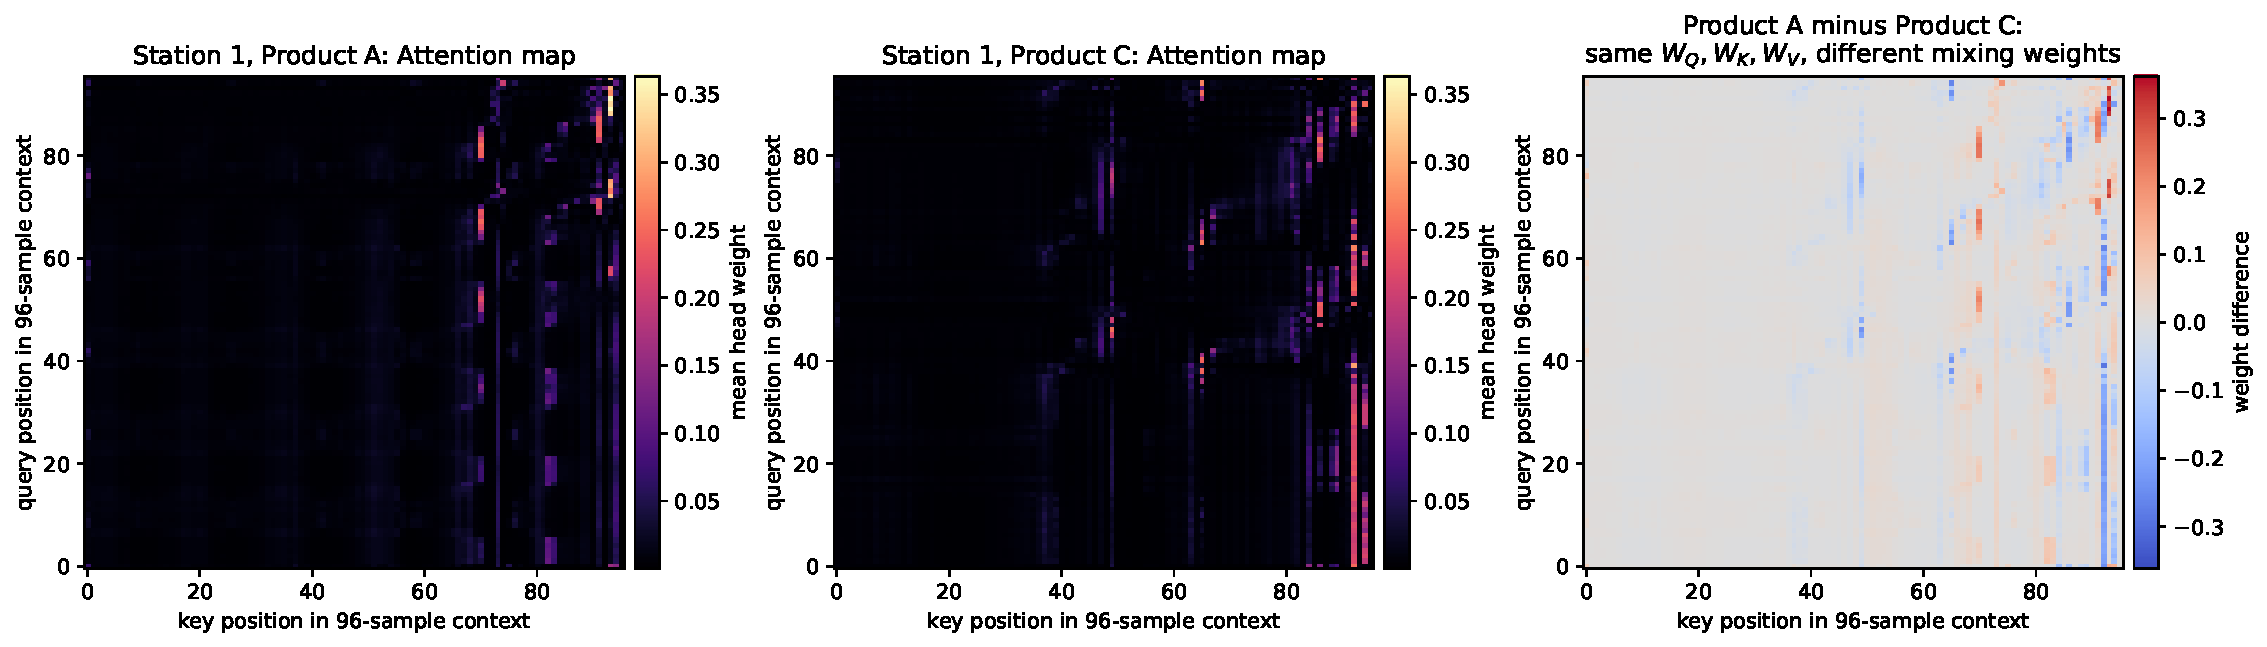
\includegraphics[width=1\linewidth]{figures/1.3-1.pdf}
\caption{Output 1.3: Raw Attention maps (mean over heads, first block) for the same two windows, and their difference.}
\end{figure}
\textbf{Same weights, different mixing} (Output 1.3, \texttt{1.3-1.pdf}: the same two windows)
\begin{itemize}
\item $W_Q$, $W_K$ and $W_V$ don't change after training, but the two contexts still give different attention maps.
\item For Product A, most of the weight goes to key positions $\approx$70, $\approx$82 and 91--94. For Product C it goes to $\approx$49, $\approx$65 and 84--94, mostly $\approx$92. The biggest absolute difference between the two maps is 0.36.
\item This happens because the scores $QK^\top/\sqrt{d_h}$ are worked out again from each window, so each context gets its own mixing matrix $\mathrm{softmax}(QK^\top/\sqrt{d_h})$, which is then applied to $V$. No refit or router is needed for this.
\item Ridge, on the other hand, applies the same $\widehat W$ to every window.
\item This only shows that the mixing depends on the input. It doesn't show that Attention found the period.
\end{itemize}

\subsection*{Response 2}
\begin{itemize}
\item \textbf{Implementation:} \texttt{SeriesDecomposition.forward} pads each end with \texttt{kernel//2} copies of the end value, runs a stride-1 average pool along time and returns $(x-T,\,T)$.
\end{itemize}
\begin{figure}[H]\centering
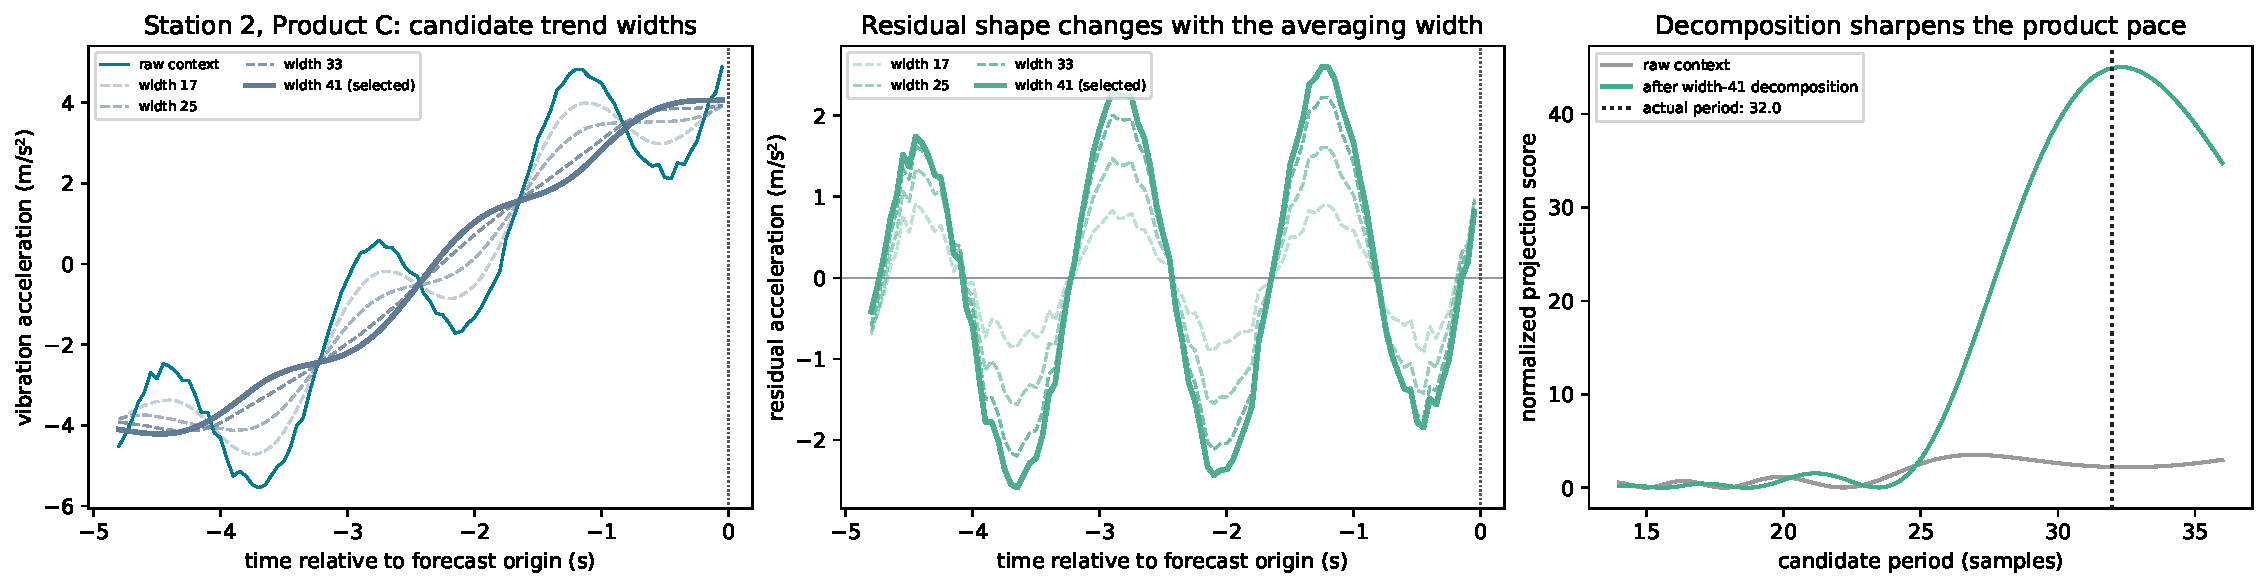
\includegraphics[width=1\linewidth]{figures/2.1-1.pdf}
\caption{Output 2.1: candidate trend widths on one validation window (station 2, Product C, $P=32$), the remainders, and the period-projection score before and after decomposition.}
\end{figure}
\textbf{Selected width: 41}
\begin{itemize}
\item \emph{Output 2.1} (\texttt{2.1-1.pdf}: one validation window from station 2, Product C, $P=32$). At width 17 the trend still follows part of the vibration, so what is left keeps only about $\pm0.9$\,m/s$^2$ of the cycle. At width 41 the trend is a smooth drift curve and what is left is a clean $\pm2.6$\,m/s$^2$ cycle around zero. Repeating the end values flattens the trend over the last $\sim$20 samples. The projection score at the true period goes up from about 2 to about 45.
\item \emph{Output 2.2} (training windows, stations 1--3). The share of contexts whose period is found within one sample goes from 0.687 (raw) to 0.980, 0.989, 0.993 and 0.998 for widths 17, 25, 33 and 41. Width 41 does have the largest median period error of the four (0.216 samples).
\item \emph{Output 2.3} (validation). Adding decomposition to Raw Attention lowers the RMSE from 0.432 to 0.305 ($-29$\%) on the established stations and from 0.649 to 0.455 ($-30$\%) on station 4, and every product gets better on both populations.
\end{itemize}
\textbf{Why a moving average makes sense here}
\begin{itemize}
\item The slow part changes over about 240 samples, while the vibration repeats every 14--36 samples.
\item A centred moving average is a simple smoothing filter with nothing to learn. At width 41 it smooths away the vibration but keeps the drift, so the drift goes into $T$ and the cycle stays in $x-T$.
\item The trend head then handles the the drift, and the mixer only has to deal with the repeating part.
\end{itemize}
\textbf{Why the oracle diagnostic is a good way to pick the width}
\begin{itemize}
\item The width's job is to make the repetition easy to see.
\item The generator knows the true period, so I can score exactly that on training windows, without touching validation, test or station-4 data and without training a network for every width.
\item It measures the decomposition itself, and not an end-to-end error that also has training noise in it.
\end{itemize}
\textbf{Where it fails}
\begin{itemize}
\item The moving average assumes the slow part is smooth inside the window. A sudden level change in the context, like a load step or a recalibration, gets spread into a 41-sample ramp, and what is left gets a half-step bump that the mixer would treat as repetition.
\end{itemize}

\subsection*{Response 3}
\begin{itemize}
\item \textbf{Implementation:} \texttt{aggregate\_delays} builds the index $(t-\tau_j)\bmod L$ for every example and selected delay, gathers the values along time with it, and adds them up with the weights $\alpha_j$.
\item \textbf{Worked example:} it returns $z=(35, 15, 25, 25)$. For example $z_0=\tfrac34 v_3+\tfrac14 v_1=35$, so position $t$ reads $t-\tau$ and the shift goes the right way.
\end{itemize}
\begin{figure}[H]\centering
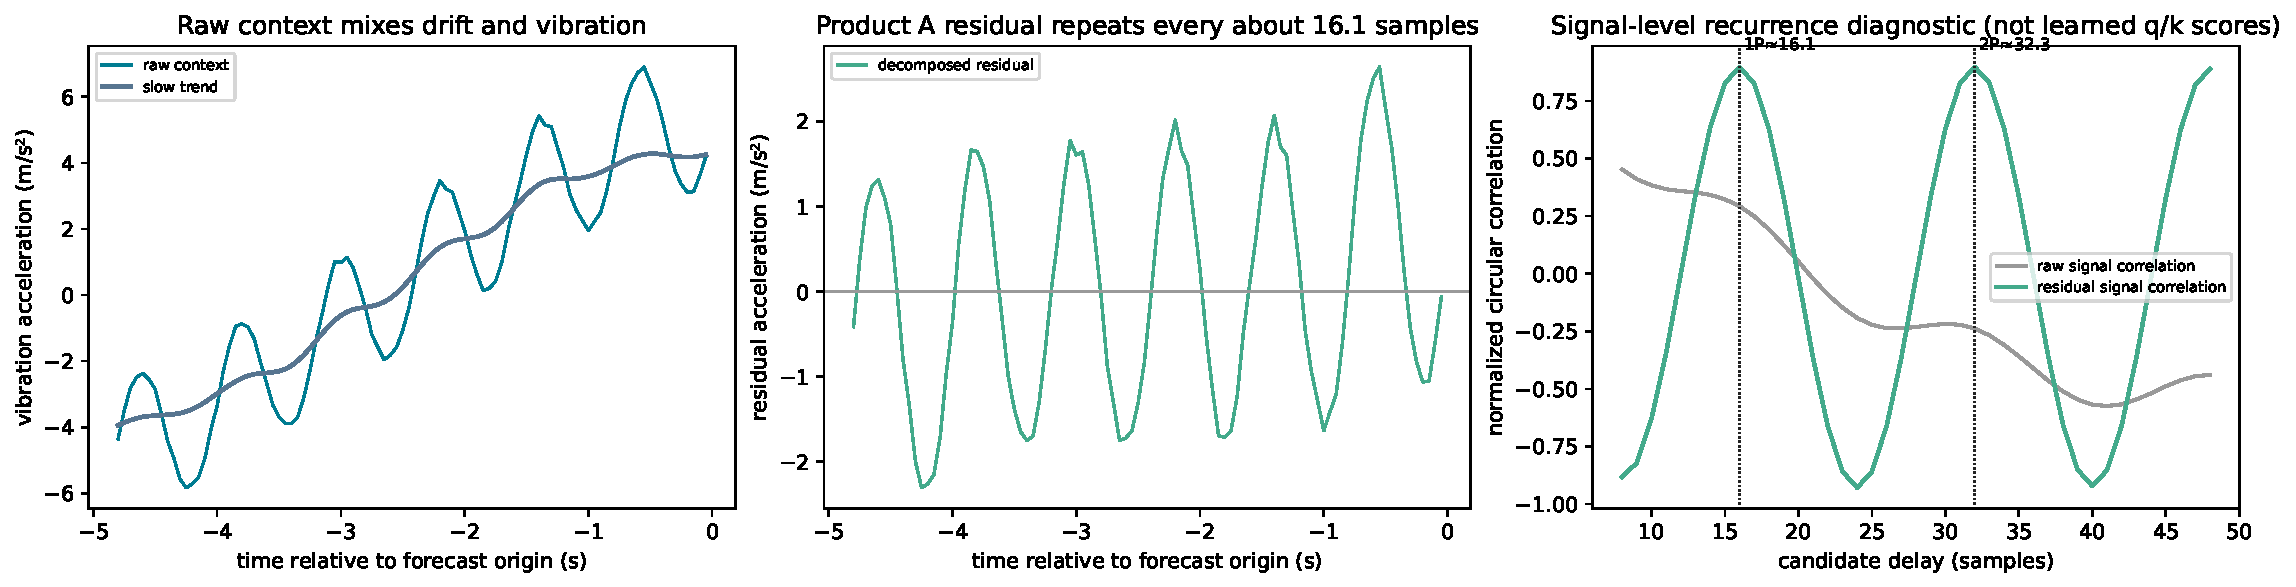
\includegraphics[width=1\linewidth]{figures/3.2-1.pdf}
\caption{Output 3.2: signal-level recurrence diagnostic on one validation window (station 2, Product A, $P=16.13$).}
\end{figure}
\textbf{Strongest lags} (Output 3.2, \texttt{3.2-1.pdf}: one validation window from station 2, Product A, $P=16.13$)
\begin{itemize}
\item The correlation of the decomposed context peaks at delays 16 ($r=0.896$) and 32 ($r=0.897$), which are the integers closest to $P$ and $2P$. It then climbs back up towards $3P\approx48.4$ at the edge of the band.
\item It is about $-0.9$ at the half-period points ($\approx$8, 24 and 40).
\item The raw signal's correlation instead just falls smoothly from 0.45 at delay 8 to about $-0.57$ near 41, with no peak at $P$ or $2P$.
\end{itemize}
\textbf{Why decomposing first helps}
\begin{itemize}
\item The raw context is a ramp of $\approx$8\,m/s$^2$ plus a $\pm$2\,m/s$^2$ cycle.
\item With circular shifts, a ramp correlates positively with itself at short delays and negatively at long ones, because the wrap joins its top to its bottom. This smooth curve hides the cycle's $\cos(2\pi\tau/P)$ part.
\item What is left after decomposition is close to zero-mean and periodic, so its correlation is roughly $\cos(2\pi\tau/P)$, with peaks at $P$ and $2P$ and a rise towards $3P$.
\item This fits what the delay mixer assumes. It scores delays, keeps a few and copies values from whole periods back, which only works if the top-scoring delays are multiples of $P$, like they are on the decomposed context.
\end{itemize}
\textbf{Where it fails}
\begin{itemize}
\item A one-off event, like a single knock from a loose part, doesn't repeat at any delay. If it is inside the context, the aggregation copies it to $t_0+\tau_j$, so the forecast gets ``ghost'' knocks one and two periods later.
\end{itemize}

\subsection*{Response 4}
\textbf{(a) Prediction, written before Output 4.1:} Decomposition should help most, because the moving average strips the drift ramp into a linear trend head before the mixer sees it. Delay mixing on its own still scores delays on the raw stream, where a large ramp correlates with itself at every lag and blurs the period evidence.

\begin{table}[H]\centering\small\setlength{\tabcolsep}{4pt}
\begin{tabular}{lrrrrrrr}
\toprule
Model & Est.\ RMSE & Est.\ MSE & $\Delta$ vs.\ Raw Attn & St.\,4 RMSE & St.\,4 MSE & Params & Fit s \\
\midrule
Shared ridge & 0.767 & 0.588 & +77\% & 0.876 & 0.767 & 4,608 & 0.002 \\
Sensor-specific ridge & 0.768 & 0.590 & +78\% & -- & -- & 13,824 & 0.072 \\
Period-routed ridge & 0.166 & 0.028 & $-$62\% & 0.173 & 0.030 & 59,904 & 0.010 \\
Raw Attention & 0.432 & 0.187 & ref. & 0.649 & 0.422 & 368,368 & 72.4 \\
Raw delay mixer & 0.225 & 0.051 & $-$48\% & 0.330 & 0.109 & 368,370 & 89.8 \\
Attention + decomposition & 0.305 & 0.093 & $-$29\% & 0.455 & 0.207 & 373,024 & 91.8 \\
Autoformer-inspired & 0.198 & 0.039 & $-$54\% & 0.244 & 0.059 & 373,026 & 109.5 \\
\bottomrule
\end{tabular}
\caption{Outputs 1.1 and 4.1: validation errors of the linear baselines and the four neural models. $\Delta$ is the change in established-station RMSE. Fit times are from the same Kaggle run, with the neural models trained on its GPU.}\label{tab:o41}
\end{table}
\begin{figure}[H]\centering
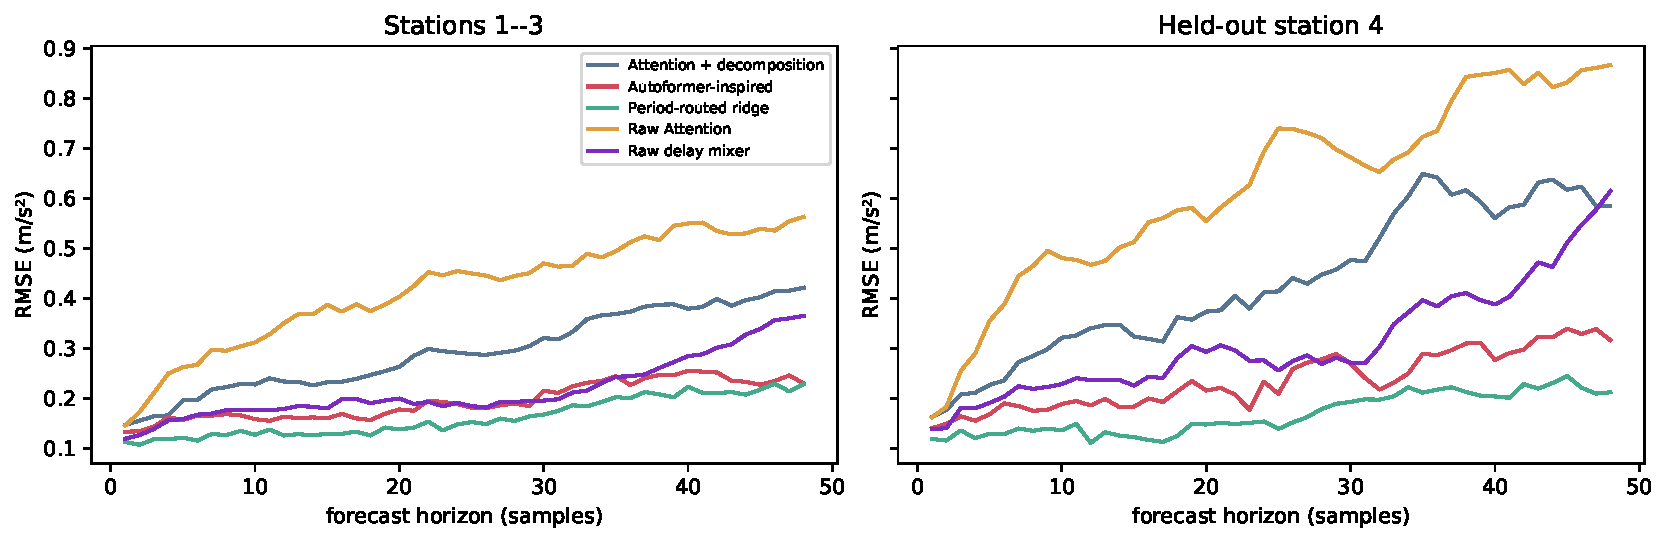
\includegraphics[width=0.8\linewidth]{figures/4.2-1.pdf}
\caption{Output 4.2: validation RMSE along the 48-step horizon, established stations (left) and station 4 (right).}
\end{figure}
\textbf{(b) Established stations, validation (Table~\ref{tab:o41})}
\begin{itemize}
\item From Raw Attention (RMSE 0.432), delay mixing alone gives 0.225 ($-48$\%), decomposition alone 0.305 ($-29$\%) and both 0.198 ($-54$\%).
\item Delay mixing helps more than decomposition in both settings ($-48$\% and $-35$\% vs.\ $-29$\% and $-12$\%), and the gains overlap instead of adding up.
\item Error grows along the horizon (Output 4.2, \texttt{4.2-1.pdf}). Routed ridge is lowest at every step (0.112 to 0.228), and Raw Attention grows fastest (0.145 to 0.563).
\end{itemize}
\textbf{(c) Deployment: period-routed ridge for both populations}
\begin{itemize}
\item It has the lowest validation MSE (0.028 established, 0.030 station 4), about 6$\times$ fewer parameters, and fits in under a second instead of 1--2 minutes.
\item The best neural model's RMSE is 19\% (established) and 41\% (station 4) higher. Being linear, it handles station 4's bigger vibrations.
\item Test RMSE (Output 4.3): 0.161 established, 0.183 station 4.
\end{itemize}

\section{Task 2 -- Leaderboard forecast with Autoformer}
\textbf{Finding the period and making features}
\begin{itemize}
\item There are no timestamps, so I had to find the period from the data itself. The periodogram (figure \texttt{t2\_periodicity.pdf}, made by \texttt{q2.py eda}) has its sharpest peak at 24.0 steps and a smaller one at 12. Nothing stands out at 168 steps, where the autocorrelation is only 0.03.
\item So I added $\sin$ and $\cos$ of $2\pi t/24$ and $4\pi t/24$ as time features. This assumes the 24-step cycle stays the same over the whole series, which the sharp peak suggests.
\item There is also a broad peak around 9,800 steps, but that is much longer than any input window, so I left it out.
\end{itemize}
\begin{figure}[H]\centering
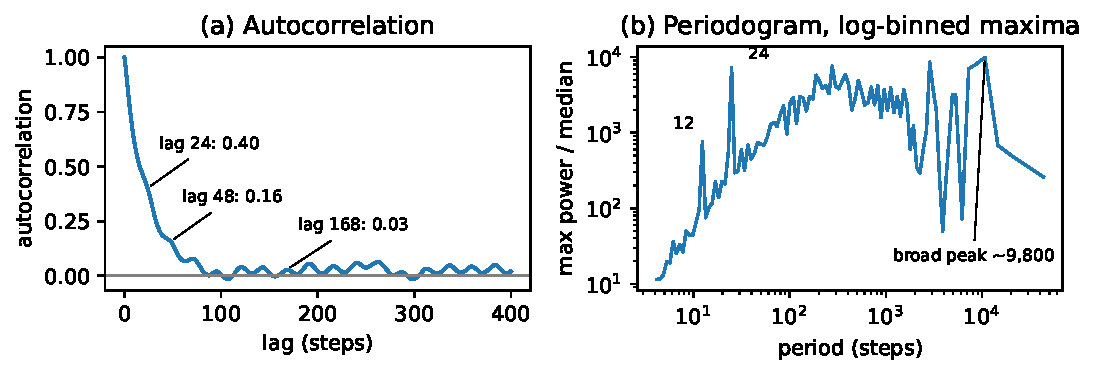
\includegraphics[width=0.9\linewidth]{figures/t2_periodicity.pdf}
\caption{Autocorrelation of the target and its periodogram (maximum power in log-spaced period bins).}
\end{figure}
\textbf{Scaling}
\begin{itemize}
\item I scaled the target with the mean and standard deviation of the training part, and didn't log-transform it, since the leaderboard scores RMSE on the raw scale.
\item I didn't normalise each window by its own mean and standard deviation. That way the model still sees the real level of the series, which I wanted becuase a simple decay back to the training mean was already a decent forecast (see the trend start below).
\item For the optional variables, I scaled A, B and C the same way. D, E and F are never negative and have a long right tail, so I took $\log(1+x)$ first. G--J are one-hot, so I left them as they are. All scaling statistics come from the training part.
\end{itemize}
\textbf{Validation}
\begin{itemize}
\item Training part: steps 1--34,920. Validation: 176 forecast origins, one every 24 steps from step 34,920 to 39,120, each scored on the next 168 steps. The last 4,368 steps (39,289--43,656) are only used in the final refit.
\item Every validation block starts at the same point of the 24-step cycle as the leaderboard block (43,656 is a multiple of 24).
\item RMSE is computed per 168-step block, like on the leaderboard, and then averaged over the blocks. MAE and sMAPE are averaged over all forecast points.
\item I made all model choices and did early stopping on this split only.
\end{itemize}
\textbf{Model} (\texttt{autoformer.py})
\begin{itemize}
\item I wrote it from scratch following Wu et al.\ (2021), reusing my Task 1 decomposition and delay aggregation.
\item \emph{Series decomposition:} a width-25 moving average, with the end values repeated at the edges, after every Auto-Correlation and feed-forward block in both the encoder and the decoder. So the trend is split off again inside every block, not just once at the start, and the decoder adds up the trend pieces it removes through a small projection.
\item Width 25 covers about one full 24-step cycle, so the cycle averages out of the trend. It also assumes the trend is smooth over that span, so a sudden jump in the level gets smeared over 25 steps.
\item \emph{Auto-Correlation:} $Q$ and $K$ are projected, and their circular cross-correlation over all lags is computed with FFTs. The model keeps the $\lfloor c\ln L\rfloor=5$ biggest lags per example ($c=1$; $L=168$ in the encoder and 252 in the decoder), turns their scores into weights with a softmax, and adds up copies of $V$ shifted by those delays (position $t$ reads $t-\tau$, like in Task 1). In the decoder's cross-correlation, keys and values are zero-padded to the query length, as in the reference code.
\item I think 5 lags is enough here, since the series really has one cycle (24 steps, plus its harmonic at 12).
\item Delay mixing can only copy patterns that repeat. Most of this series isn't periodic (the autocorrelation is close to 0 after about 100 steps), so I didn't expect the past values alone to predict its big jumps.
\item \emph{Encoder--decoder:} input 168 steps, label 84, \texttt{pred\_len}=168, one encoder layer and one decoder layer, $d=16$, 2 heads, $d_{ff}=32$, dropout 0.05. I kept it small because the score penalises parameters.
\item All 168 steps come out in one shot, so mistakes in the early steps aren't fed back in as inputs for later steps.
\item The value is embedded with a width-3 convolution, and the time features and optional variables go in as marks through a linear layer.
\item \emph{Trend start:} the paper starts the horizon trend at the window mean. The autocorrelation drops from 0.97 at lag 1 to 0.40 at lag 24, so the last value says a lot about the next few steps and less after that. So I start the trend at a decay from the last value $y_t$ back to the training mean $\mu$, $\mu+(y_t-\mu)e^{-h/\tau}$, with learned weights on the last value and on the window mean for each horizon step $h$ (336 parameters).
\item $\tau=24$ gave the lowest validation RMSE (81.6) out of $\{6,12,24,48\}$ when I used this formula on its own as a forecast (\texttt{q2.py tau}).
\end{itemize}
\textbf{Training}
\begin{itemize}
\item MSE on the scaled target, Adam with learning rate $10^{-3}$ halved every epoch (as in the Autoformer code), batch 64 and gradient clipping at 1.
\item One epoch is one pass over every stride-1 window of the training part.
\item Early stopping on validation RMSE, with patience 2 and at most 6 epochs.
\end{itemize}

\begin{table}[H]\centering\small
\begin{tabular}{lrrrr}
\toprule
Optional variables & P & MAE & RMSE & sMAPE \\
\midrule
none & 6,001 & 65.2 $\pm$ 0.2 & 80.5 $\pm$ 0.2 & 67.4 $\pm$ 0.1 \\
past only (encoder marks) & 6,161 & 65.4 $\pm$ 0.7 & 80.7 $\pm$ 0.5 & 67.5 $\pm$ 0.5 \\
past and future (encoder and decoder marks) & 6,321 & 48.6 $\pm$ 0.5 & 63.1 $\pm$ 1.3 & 64.3 $\pm$ 0.6 \\
past and future, clipped at 11 & 6,321 & 47.7 $\pm$ 0.5 & 62.7 $\pm$ 1.3 & 51.8 $\pm$ 0.5 \\
\bottomrule
\end{tabular}
\caption{Validation results with and without the optional file, mean $\pm$ sd over seeds 0, 1 and 2. All rows use the time features. Forecasts are clipped at 0, except in the last row; clipping the first two rows at 11 changes them by less than 0.01.}\label{tab:abl}
\end{table}
\textbf{What the optional file did (Table~\ref{tab:abl})}
\begin{itemize}
\item It helps, but only through its values over the horizon. With them, validation RMSE drops from 80.5 to 63.1 ($-22$\%) and MAE from 65.2 to 48.6, and all three seeds with them beat all three without them.
\item Giving the model only the values up to the forecast origin does nothing (80.7 vs.\ 80.5). So the variables belong in the decoder marks, where each forecast step sees its own conditions, and not only in the encoder.
\item Without the optional file, the Autoformer is only about 1 point better than the decay formula on its own (80.5 vs.\ 81.6). So from its own history alone, this series doesn't gain much from a bigger model. The optional variables are what made the Autoformer worth it.
\item The metrics disagree. RMSE and MAE drop by 22--25\%, but sMAPE only goes from 67.4 to 64.3. The reason is forecasts of zero: 7--8\% of this model's raw validation outputs are negative and get clipped to 0, and a forecast of 0 always scores the maximum sMAPE of 200\%, while RMSE and MAE barely notice it. Clipping at 11 instead (the 5th percentile of the training values, not tuned) brings sMAPE down to 51.8 and also lowers RMSE and MAE a bit (last row).
\item Which variables matter: shuffling one variable accross the 176 validation origins (input window and horizon together; 3 seeds $\times$ 3 shuffles) raises RMSE by 31 for A and 42 for B, by 5.4 for G--J together, and by only 0.5--2.7 for C, D, E and F. So almost all of the signal is in A and B.
\end{itemize}
\textbf{Final model and submission}
\begin{itemize}
\item Seed 0's validation run had its best RMSE after epoch 2 and stopped at epoch 4.
\item I refit the same model (past and future marks) from scratch on all 43,656 steps for 2 epochs, with no early stopping, and clipped the forecast at 11 like above.
\item $P=6{,}321$ trainable parameters. Following Section 2.7 of the brief, $E$ counts both the early-stopped run and the refit, so $E=4+2=6$.
\item \texttt{python q2.py final 0} reads seed 0's validation run from \texttt{results/runs.csv}, reproduces the forecast (\texttt{results/forecast.txt}) and writes $P$ and $E$ to \texttt{results/final.json}.
\end{itemize}
\textbf{Reference:} H.~Wu, J.~Xu, J.~Wang and M.~Long, ``Autoformer: Decomposition Transformers with Auto-Correlation for Long-Term Series Forecasting,'' NeurIPS 2021.\\ Official code: \url{https://github.com/thuml/Autoformer}.

\section*{Appendix: Use of generative AI}
I used Claude (Anthropic) as a drafting helper and guide. The prompts and outputs are mentioned below:
\begin{enumerate}[leftmargin=1.5em]
\item \textbf{Prompts:} {\itshape guide me on how do I run this assignment on mps instead of cpu - i have a mac m3 max with 30-core gpu}\\
{\itshape Is running on Kaggle better?}\\
\textbf{Output:} instructions for running it on an Apple GPU (MPS), and a comparison with running it on Kaggle. informed about compatibility issues, suggested Kaggle.
\item \textbf{Prompt:} {\itshape i tried running this on kaggle as well but it's looking for harness folder (not finding it)? how do I add that folder to kaggle}\\
\textbf{Output:} explanation on using os library for changing directory and uploading zip as a dataset
\item \textbf{Prompts:} {\itshape Okay that's working fine i guess, we'll see when it finishes. I also need to work on the report thing. As written in the manual attached too, I need to work on this report to elaborate on the work I did. I am attaching the figures that I need to refer in the assignment - how do you think is the best way to structure this? I do not want to write a load of content so what's the best way of answering the responses with minimal effort}\\
\textbf{Output:} the list of deliverables and report requirements from the handout, bulleted structure with references to figures and citations to used work
\item \textbf{Prompts:} {\itshape can you give me like a draft skeleton of the report structure that i can edit with my content and findings?}\\
\textbf{Output:} sample LaTeX file with key headlines and elements to explain the ideal structure and requirements for each task
\end{enumerate}
\end{document}
